\chapter[Engenharia de Requisitos]{Engenharia de Requisitos}
Na seção a seguir será dada uma pequena introdução dos três níveis de projeto do SAFe (Portfolio, Program, Team), e será dito um pouco sobre esses níveis no contexto de projeto do grupo 1. Certas adaptações foram feitas com base nas características dos integrantes de ambos os grupos (Requisitos e MPR). Então, na seção seguinte (\emph{Papéis}) será falado sobre os papeis principais do SAFe no contexto do grupo. Certos papeis foram retirados (por serem julgados como desnecessários para o contexto do projeto), e, portanto, não serão citados nem explicados. Papeis utilizados serão explicados, e, caso eles sejam alterados para que funcionem de maneira diferente à referida na bibliografia, essas alterações serão explicadas e justificadas.

\section{Scaled Agile Framework}
\subsection{Nível de Portfólio}
\begin{figure}[h]
  \centering
  \caption{Nível de Portfólio no SAFe - \cite[p. 44]{safe001}}
  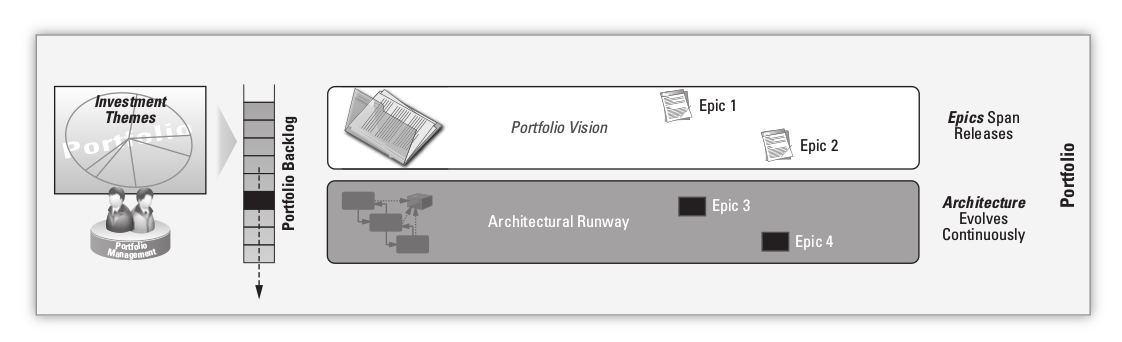
\includegraphics[width=400px, scale=0.5]{figuras/PortfolioLevel.ps}
\end{figure}

Responsável pelos artefatos \emph{epics} e \emph{investiment themes}, este nível de projeto traz os requisitos com maior nível de abstração dentre os três níveis. Contém um tipo de time (\emph{portfolio management team}), costuma ter seu próprio backlog (\emph{portfolio backlog}), e apresenta os conceitos de \emph{portfolio vision} e de \emph{architectural runway} \cite[p. 227-228]{safe001}. No contexto do grupo 1 esse nível de projeto será bastante customizado, pois julga-se o tamanho do projeto como pequeno, fazendo-se desnecessária a utilização de certos papéis e certos conceitos (costumam ser utilizados para grandes projetos, e a não utilização de tais não prejudicará a qualidade do processo). Ao invés de se usar o \emph{portfolio backlog}, os épicos entre outros insumos nascidos nesse nível serão armazenados no \emph{program backlog}. Essa escolha foi feita pois o épico ocorre em um nível muito macro para o nível do projeto, onde o grupo voltaria a este possível \emph{backlog} pouquíssimas vezes durante o projeto. Logo preferiu uni-lo ao \emph{backlog} de Nível de Programa, deixando um papel cuidando de ambos.

\subsection{Nível de Programa}
\begin{figure}[h]
  \centering
  \caption{Nível de Programa no SAFe - \cite[p. 39]{safe001}}
  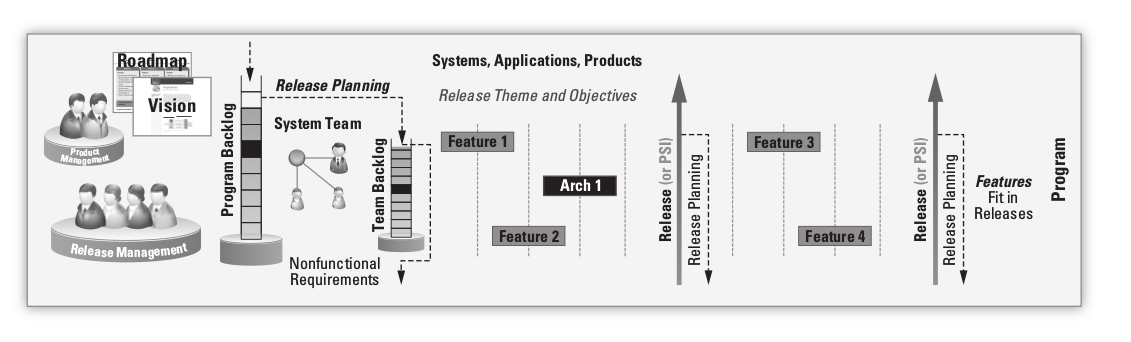
\includegraphics[width=400px, scale=0.5]{figuras/ProgramLevel.ps}
\end{figure}
Esse nível tem como principais objetivos manter a visão (Documento de Visão), gerenciar a \emph{release}, gerenciar a qualidade (integrando os resultados obtidos pelos times, e garantindo que os padrões de qualidade, performance, entre outros, estão sendo assegurados), fazer o \emph{deploy} do sistema, gerenciar recursos (ajustando prazo e gastos), entre outras tarefas \cite[p. 63-64]{safe001}. No contexto do grupo 1, os integrantes de MPR fornecerão dados para a escrita das \emph{features} (principalmente sob o papel de PO, já que não será utilizado o papel de PM), os alunos de Requisitos escreverão as features e as documentarão no Documento de Visão. Como já dito, haverá o \emph{program backlog}, onde serão armazenadas \emph{features}, épicos, entre outras coisas.

\subsection{Nível de Time}
\begin{figure}[h]
  \centering
  \caption{Nível de Time no SAFe - \cite[p. 34]{safe001}}
  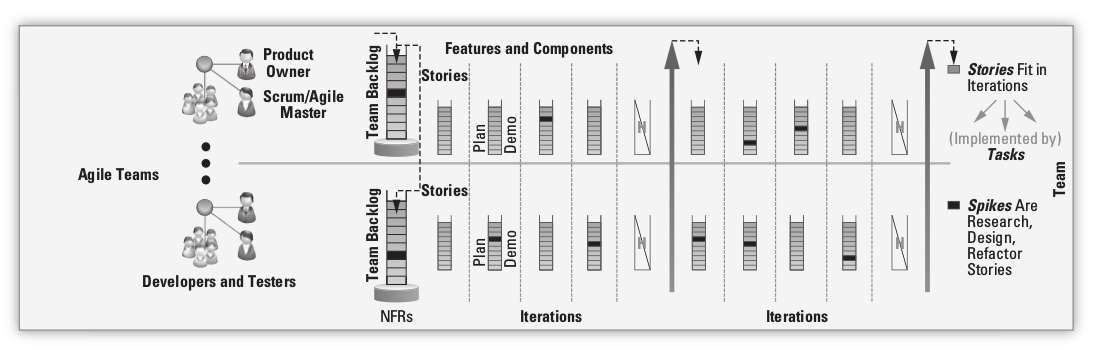
\includegraphics[width=400px, scale=0.5]{figuras/TeamLevel.ps}
\end{figure}
A unidade básica de trabalho para este nível é a \emph{estória de usuário}. O objetivo deste nível é definir, construir e testar as estórias de usuário no escopo de uma \emph{sprint}, afim de se concluir mais partes do produto final \cite[p. 47-48]{safe001}. No contexto do grupo 1, os alunos de MPR terão o papel de \emph{product owner}, fornecendo os insumos necessários para a escrita das estórias, que serão escritas em conjunto entre PO e desenvolvedores. Além disso, os alunos de Requisitos farão todo o processo de alimentação do \emph{backlog} de time, processo de planejamento da \emph{sprint} (serão os \emph{Scrum Masters}), priorização das estórias com base no WSJF, desenvolverão e testarão as soluções (com base nos critérios de aceitação).

\section{Papéis}
Um papel define comportamentos e responsabilidades de um indivíduo ou de um grupo de indivíduos que trabalham juntos como um time \cite[p. 61-65]{kruchten001}. O corportamento é expresso em termos de atividades que o papel pratica, e, cada papel é associado a um conjunto de atividades. No SAFe existem diferentes papéis para os diferentes níveis do sistema. No Nível de Portfólio vão haver, principalmente, papéis que irão interagir com os épicos e temas de investimento, no Nível de Programa, papéis que irão interagir com as \emph{features}, e, no Nível de Time, papéis que irão interagir com estórias de usuário.

Nesta seção será dada uma breve definição de papeis que serão utilizados, justificativas e explicações para papeis customizados, e quem representa este papel no contexto do grupo 1.

\subsection{Papéis no Nível de Portfólio}
\subsubsection{Epic Owner}
Responsável por definir e analisar o trabalho que será seguido no épico \cite[p. 418-419]{safe001}. No contexto do grupo 1, afim de não descaracterizar a estrutura do SAFe, este papel terá o papel de gerenciar o Nível de Portfólio e de ser o responsável pelos épicos.

% \subsubsection{Enterprise Architect}
% Responsável por manter um alto nível/visão holística da empresa e das iniciativas de desenvolvimento, participa na estratégia de construir e manter o \emph{Architectural Runway}, entender os temas estratégicos, dirigir o \emph{Architectural Epic Kanban} entre outras tarefas \cite{safesite001}.

\subsection{Papéis no Nível de Programa}

\subsubsection{Product Manager}
Responsável por entender as necessidades do cliente, documentar, priorizar e validar requisitos (no nível de \emph{feature}), gerenciar mudanças, entre outras coisas \cite[p. 283-287]{safe001}. No contexto do grupo 1, o Gerente do Produto (\emph{product manager}, PM) não será utilizado e algumas de suas tarefas serão atribuidas a outros papéis, pois uma de suas principais atribuições é a de gerenciar os diversos PO's, quando existem. Como no contexto do grupo haverá apenas um PO, as tarefas do PM serão atribuidas ao PO, e este papel deixará de existir. % Ele Será o responsável por entender as necessidades do cliente e transferir esse conhecimento adquirido para a equipe quem escreverá as \emph{features} e as estórias de usuário. Não cuidará do \emph{program backlog} (diferente do sugerido pela bibliografia), nem fiscalizará os \emph{Product Owners}. Todas essas mudanças ocorreram para poder adaptar o papel de PM ao máximo para integrantes da disciplina de MPR. As atividades mais ligadas aos alunos de Requisitos (escrever a \emph{feature}, cuidar do \emph{program backlog}, validar requisitos) ficarão com outros papeis, restritos aos alunos de Requisitos.

\subsubsection{Release Management}
Consistindo do Product Manager e do Release Train Engineer, o papel de Release Management é responsavel por comunicar o \emph{status} da release aos \emph{stakeholders}, coordenar com a gerência do produto e gerência de \emph{marketing} as comunicações internas e externas, validar a qualidade relevante do produto de acordo com critérios, prover a autorização final da \emph{release}, ajudar a adaptar e inspecionar o processo de \emph{release}, entre outras coisas \cite{safesite001}.
No contexto do grupo 1, o Release Management será feito somente por quem atua no papel de \emph{Release Train Engineer}, no caso, os alunos de Requisitos. O papel não será compartilhado com os alunos de MPR pois, como já dito, pratica atividades com mais relação com a disciplina de Requisitos. Será um papel flutuante, onde cada semana um aluno do grupo terá o papel de ser /emph{release manager}.

\subsubsection{Business Owners}
Pequeno grupo de \emph{stakeholders} de grande confiança, que dispõe de capacidade de administração, responsáveis pela gestão, qualidade, implantação e desenvolvimento de software \cite{safesite001}. No contexto do projeto, diferente da bibliografia, eles não serão responsáveis pelo desenvolvimento e implantação do \emph{software}, e será praticado pelos alunos de MPR.

%\subsubsection{Release Train Engineer}
%\subsubsection{UX}
%\subsubsection{Shared Resources}

\subsection{Papéis no Nível de Time}

\subsubsection{Product Owner}
Responsável por representar o interesse de todos os envolvidos no projeto, faz parte do time e esta junto no dia-a-dia dos desenvolvedores e testadores, elaborando as estórias de usuário e ajudando o time a alcançar seus objetivos \cite[p. 47-48]{safe001} Além de ser um membro que possui visão do modelo de negócio. No contexto do grupo 1, o \emph{product owner} não irá escrever as estórias. O papel de PO será delegado a um integrante de MPR que deverá validar e analisar a escrita das estórias que será feita pelos integrantes do grupo de Requisitos.

\subsubsection{Scrum Master}
É responsável por facilitar o progresso do time (ajudando assim a se alcançar o objetivo final), liderar os esforços do time, reforçar as regras do processo ágil e eliminar impedimentos \cite[p. 47-48]{safe001}. No contexto do grupo 1, o papel de \emph{Scrum Master} irá flutuar durante o projeto, e será escolhido um integrante do grupo de Requisitos para ser \emph{Scrum Master} a cada \emph{sprint}. Essa rotatividade irá fazer com que todos os integrantes aprendam a ser um \emph{Scrum Master}, e, só é necessário um por \emph{sprint}.

\subsubsection{Desenvolvedores e Testadores}
Responsáveis por desenvolverem e testarem as estórias de usuário. No contexto do grupo 1, todos os integrantes de Requisitos farão parte desse papel, e também será responsável por escrever as estórias de usuário e os critérios de aceitação. Este papel ainda será responsável pelo desenvolvimento da solução final e por testar as estórias.


\section{Atividades}
Serão detalhadas nessa seção o conjunto de atividades a serem feitas durante o projeto, e quem está envolvido na atividade.
Modelagem geral de atividades:

\begin{figure}[h]
  \centering
  \caption{Modelagem das atividades, feita no \emph{Bizagi}}
  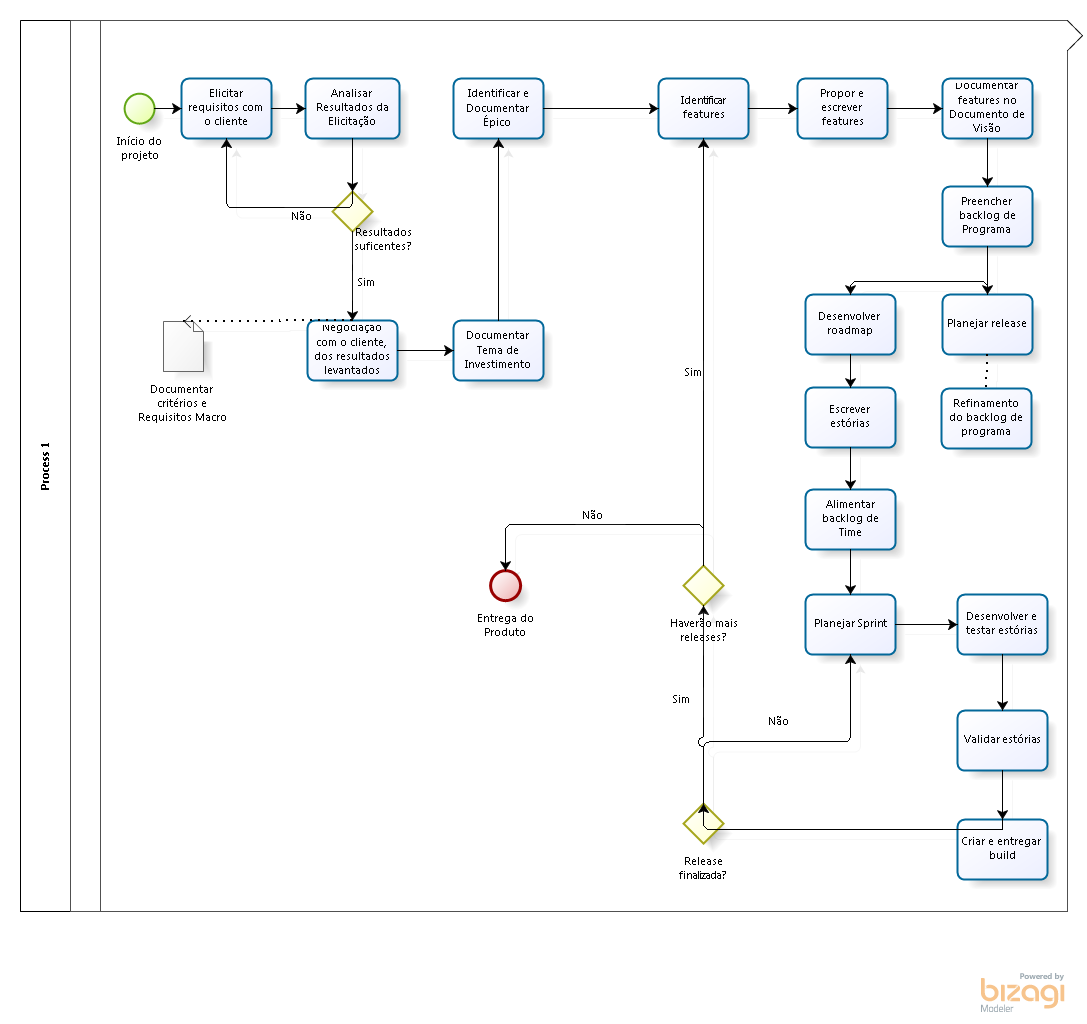
\includegraphics[width=400px, scale=0.5]{figuras/ModelagemInicial3.ps}
\end{figure}

Lista de atividades:
\begin{itemize}
  \item Elicitar requisitos com o cliente: no contexto do grupo 1, atividade feita pelo \emph{epic owner} (Requisitos) e cliente (MPR), consiste em entender de maneira macro o contexto e as necessidades do projeto.
  \item Analisar resultados da elicitação: Atividade feita pelos \emph{epic owners}, consiste em se analisar os insumos fornecidos pelo cliente na atividade anterior, buscando-se soluções plausíveis e pontos de vista diferentes.
  \item Negociação com o cliente dos resultados levantados: feita entre \emph{epic owner} e cliente, consiste em expor os pontos de vista descobertos na análise, tentando encontrar um ponto comum entre a visão do cliente e da equipe.
  \item Documentar critérios e requisitos: documentar de maneira formal as necessidades e descrições necessárias no projeto conseguidos na negociação, tudo em um nível bem macro. Feito pelo \emph{epic owner}, guiará a visão do épico.
  \item Identificar \emph{features}: consiste em identificar as possíveis \emph{features} do sistema. Feita em conjunto entre o \emph{Product Owner} (que, como já dito, no contexto do grupo 1 terá as tarefas do PM) e o RTE (alunos de Requisitos), será salva no \emph{backlog} de programa.
  \item Propor e escrever features: com as possíveis \emph{features} identificadas, se chega a um ponto comum se tal \emph{feature} deve estar presente ou não. Se sim, serão escritas e salvas. Feito em conjunto entre o PO e o RTE.
  \item Documentar \emph{features} no Documento de Visão: Feito pelo RTE (alunos de Requisitos), consiste em documentar as \emph{features} levantadas no Documento de Visão.
  \item Preencher \emph{backlog} de programa: consiste em documentar o conjunto de \emph{features} disponíveis no \emph{backlog} de programa, dando assim uma melhor visão para o time de qual solução pode ser implementada em determinado momento. Feita pelo Release Manager.
  \item Planejar \emph{release}: consiste em definir quais \emph{features} serão implementadas na \emph{release}, períodos, visões, etc. Feita em conjunto entre os papéis de Release Manager, PO e RTE.
  \item Refinamento do \emph{backlog} de programa: Consiste principalmente em dizer o estado atual de cada \emph{feature} que deve ser implementada na \emph{release} atual. Tarefa feita pelo Release Manager.
  \item Escrever estórias de usuário: consiste em documentar as estórias de usuário advindas de uma determinada \emph{feature}. Feita em conjunto entre PO, Desenvolvedores e Scrum Master.
  \item Alimentar \emph{backlog} de time: consiste em documentar e armazenar o conjunto de estórias no backlog, garantindo também sua rastreabilidade. Feito pelo Scrum Master.
  \item Planejar \emph{sprint}: Feito em conjunto entre PO, Desenvolvedores e Scrum Master, consiste em planejar o que será implementado na \emph{sprint} seguinte, quem fica com determinada tarefa, pontos falhos da \emph{sprint} passada, etc.
  \item Desenvolver e testar estórias: tarefa feita pelos desenvolvedores e testadores, consiste em desenvolver determinada estória de usuário, testar e validar com base nos critérios de aceitação.
  \item Criar e entregar \emph{build}: Feita pelos desenvolvedores, consiste em empacotar o desenvolvimento das estórias feitas numa determinada sprint, transformar em produto, e entregar este incremento ao usuário.
\end{itemize}

